\section{The LHCb detector}
\label{sec:Detector}
Alongside ALICE, ATLAS and CMS, LHCb is one of the four main experiments located at the Large Hadron Collider (LHC) at CERN. At the LHC, opposing proton beams are brought to
collision at the four main interaction points with a bunch collision rate of $\qty{40}{\mega\hertz}$. The resulting particle cascades can then be measured and analysed using the
different experiments. LHCb is designed to measure decays including $b$ and $c$ quarks which play an important role in the field of \textit{CP} violation. 

The detector is a single-arm forward spectrometer with an acceptance of $2 \leq \eta \leq 5$ in the pseudorapidity range. A schematic view of the apparatus as used in the data taking
period relevant for this analysis can be seen in \autoref{fig:lhcb_detector}.
\begin{figure}
    \centering
    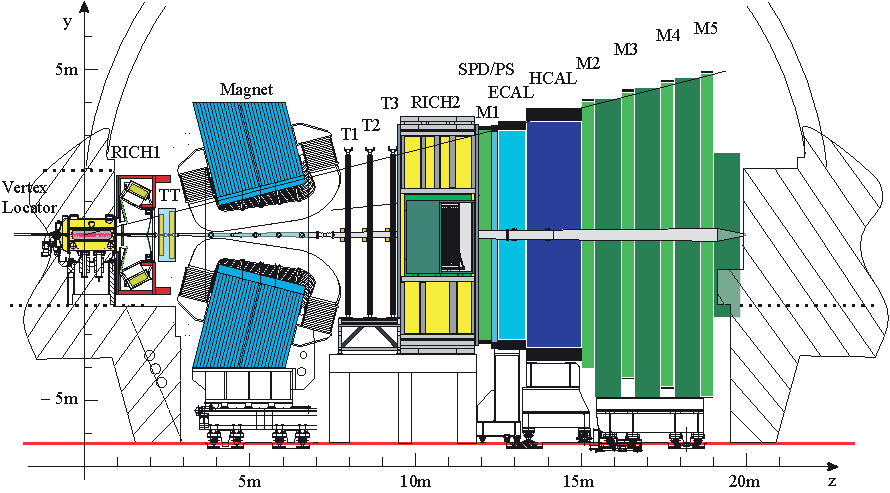
\includegraphics[width = .8\textwidth]{"content/pics/LHCb-Detektor.pdf"}
    \caption{The setup of the Large Hadron Collider beauty experiment as used in Run~1~\cite{LHCb_detector}. 
    The collision point of the protons is on the left. The Vertex Locator (VELO),
    the tracking stations (TT, T1-T3), the Ring Imaging Cherenkov detectors (RICH1-2), as well as the calorimeters (SPD/PS, ECAL, HCAL) and the muon chambers (M1-M5) can be seen.}
    \label{fig:lhcb_detector}
\end{figure}
The interaction point of the proton-proton collisions is located at the very left of the graphic, at the Vertex Locator (VELO). The VELO's primary purpose is to 
measure the primary and secondary vertices of decays. It therefore needs to provide a high spatial resolution. This information can then be used to reconstruct the lifetime and
impact paramter (IP) of the decays. \mbox{$B$-mesons}, for example, typically decay after a few $\unit{\milli\metre}$ to $\unit{\centi\metre}$ and can therefore be measured in 
the VELO. 
The tracking stations TT (Tracker Turicensis) and T1-T3 are used to reconstruct tracks of (charged) particles deflected by the dipole magnet, 
which has an integrated field strength of $\qty{4}{\tesla\metre}$. The information from the tracking stations can be used to calculate momentum and charge of a particle.
The Ring Imaging Cherenkov detectors RICH~1~and~2 lie upstream and downstream of the tracking stations, respectively. 
Here, the velocity of traversing particles is calculated from diameter measurements of light cones caused by the Cherenkov effect. 
Together with the momentum information, this contributes to the particle identification (PID) and can be used to determine kaons from pions. 
Further downstream, the calorimeter system consisting of the Scintillating Pad Detector (SPD), the Preshower detector (PS) and the electromagnetic- (ECAL) and 
hadronic (HCAL) calorimeters is located. The calorimeters are utilised to measure the particles energy deposition and also contribute to PID.
At the very end of the detector, the muon chambers (M1-M5) measure muons which do not interact much with the aforementioned detector parts. \\
Events measured by the detector are triggered and preprocessed by a three-level trigger system. The reconstructed decays of interest are then saved to storage for further offline 
analysis. 

\section{Analysis strategy}
\label{sec:Analysis_strategy}
The data used for this analysis was taken in 2011 at a center of mass energy of $\qty{7}{\tera\eV}$. It includes $\num{3.4}(\num{5.1})$ million events of 
$B^{\pm} \to h^{\pm} h^+ h^-$ decays ($h^{\pm}$: hadron; kaon $K^{\pm}$/ pion {$\pi^{\pm}$}) with dipole magnet polarity up (down), 
corresponding to an integrated luminosity of $\qty{434}{\pico\barn^{-1}}$ ($\qty{584}{\pico\barn^{-1}}$) \cite{LHCb_CPV}. 
Here, only the decay into three kaons ($h^{\pm} =  K^{\pm}$) is considered.
A dataset of simulated $B^{\pm} \to K^{\pm} K^+ K^-$ decays is also available. \\
At first, the data is read from the provided \texttt{.root} files using the python extension \textit{pyROOT} of the software package \textit{ROOT} \cite{ROOT}.
Histograms of the distributions of the variables listed in the file are to be created for the simulated and measured data. The provided parameters for both simulation
and real data are listed in the appendix. The simulated data does not include decays via resonances.
Next, the energy of the kaons in the simulated data is calculated using the known kaon mass and its momentum. From this, the invariant mass of the $B$-mesons can be calculated 
and histogrammed. 
The same is done for the measured data after decays with only kaons in the final state are selected using PID information from the variables listed in the dataframe. 
A high efficiency should be maintained. The differences between the mass distributions of the measured- and simulated data are to be described.
Following that, the global \textit{CP} asymmetry, its uncertainty and significance are calculated.
In the next step, Dalitz plots are created for the simulated and experimental data. Using the Dalitz diagrams, charm resonances that are present in the measured data can be 
identified and removed. Finally, the local \textit{CP} violation in different areas of the Dalitz plot is to plotted. The areas with the most significant evidence of \textit{CP} violation 
should be identified and the significance of \textit{CP} violation in this areas should be calculated. 
